\documentclass{article}
\usepackage{graphicx}
\usepackage[russian]{babel}
\usepackage{asymptote}
\begin{document}
\begin{figure}
\centering
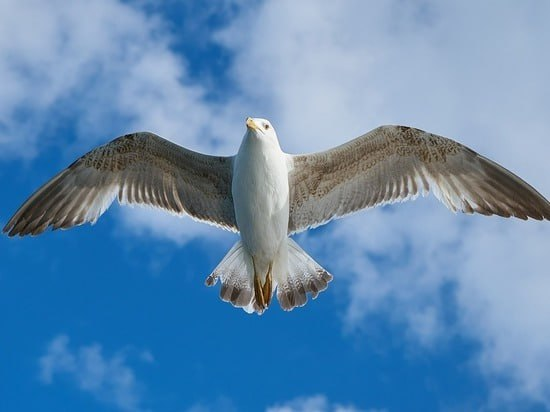
\includegraphics[scale=3]{птичка_для_теха.jpg}
\caption{ }
\end{figure}
\begin{asy}
unitsize(1.5cm);
path thebox = box((0,0),(1,1));
fill(thebox, white);
draw(shift(9.2,9.2)*thebox,green+linewidth(3pt));
clip(thebox);
path f=(0.5,-0.5)--(1.5,-0.5)--(1.5,0.5)--(0.5,0.5)--cycle;
filldraw(f,fillpen=green, drawpen=linewidth(1mm)+.99red);
path g=(0.5,0)--(1,0)--(1,0.5)--(0.5,0.5)--cycle;
filldraw(g,fillpen=blue, drawpen=linewidth(1mm)+.99red);
draw(shift(0,0)*thebox,red+linewidth(3pt));
draw(scale(.75)*Label(
"$\varnothing$",align=3.5*RightSide, position=Relative(2.75)), g,red);
\end{asy}
\end{document}